\section{Theoretical Analysis}
\label{sec:analysis}


In this section we will approach and conduct a theoretical study of an Amplifier circuit. We started by performing an operating point analysis in order to discover the values ​​of all voltages and static currents. For this purpose, the mesh method was used, through which the following equations were obtained:


%Obendo então os seguinte valores explícitos na tabala em baixo

\FloatBarrier
\begin{table}[h]
  \centering
  \begin{tabular}{|c|c|}
    \hline    
    \input{nome do ficheiro}
    \hline
  \end{tabular}
  \caption{Operating point analysis using Octave}
  \label{tab:Octave}
\end{table}
\FloatBarrier    



\par Then, gain, input and output impedances were also obtained for two different states, namely for the gain stage and the output stage.
 The equations used to compute the results for the Gain stage are as follows:

% fórmulas do slide 8 ou 12 de acordo se não tem ou tem o circuito com o bypass C - gain  

\begin{equation}
  frac{v_o}{v_i} = -g_{m}(frac{1}{R_C}+frac{1]{r_o})v_{pi}
  \label{}
\end{equation}   

where: 

\begin{equation}
  v_{pi} = frac{frac{1}{r_{pi}}+frac{1}{R_{B1}}+frac{1}{R_{B2}}}{R_{S}+(frac{1}{r_{pi}}+frac{1}{R_{B1}}+frac{1}{R_{B2}})}v_{s}
  \label{}
\end{equation}   

%  fórmulas do slide 13  

\begin{equation}
  Z_{I}=frac{1}{R_{B1}}+frac{1}{R_{B2}}+frac{1}{r_{pi}}
  \label{}
\end{equation}  

\begin{equation}
  
Z_{O}=frac{1}{R_{C}}+frac{1}{R_{o}}}
  \label{}
\end{equation}

\par In parallel, the equations involved in computing for the Output stage are as follows:

% fórmulas do slide 15 - gain  
\begin{equation}
  
frac{v_{o}}{v_{i}}=frac{g_m}{g_{pi}+g_{E}+g_{o}+g{m}}
  \label{}
\end{equation}

where g's are the admitances. 

\begin{equation}
  
Z_{I}=frac{g_{pi}+g_{E}+g_{o}+g{m}}{g_{pi}(g_{pi}+g_{E}+g_{o})}
  \label{}
\end{equation}

\begin{equation}
  
Z_{O}=frac{1}{g_{pi}+g_{E}+g_{o}+g{m}}
  \label{}
\end{equation}


% fórmulas do slide 16 - impedances 

Using the Octave software, the following values ​​were obtained:

\FloatBarrier
\begin{table}[h]
  \centering
  \begin{tabular}{|c|c|}
    \hline    
    \input{nome do ficheiro}
    \hline
  \end{tabular}
  \caption{Voltage gain, Input and Output Impedances for Gain Stage}
  \label{tab:Octave}
\end{table}
\FloatBarrier    

\FloatBarrier
\begin{table}[h]
  \centering
  \begin{tabular}{|c|c|}
    \hline    
    \input{nome do ficheiro}
    \hline
  \end{tabular}
  \caption{Volatge gain, Input and Output Impedances for Output Stage}
  \label{tab:Octave}
\end{table}
\FloatBarrier     

% As wanted the input impedance of the output stage is bigger than the output impedance of the gain stage. And thats the reason why the circuit presents very little signal loss. (explicação)

Finally, a study was carried out in the frequency domain for the incremental circuit of voltage gain, then obtaining the graph in dB or SOMETHING LIKE THIS: 


\begin{figure} [!htb] 
  \minipage{0.9\textwidth}
  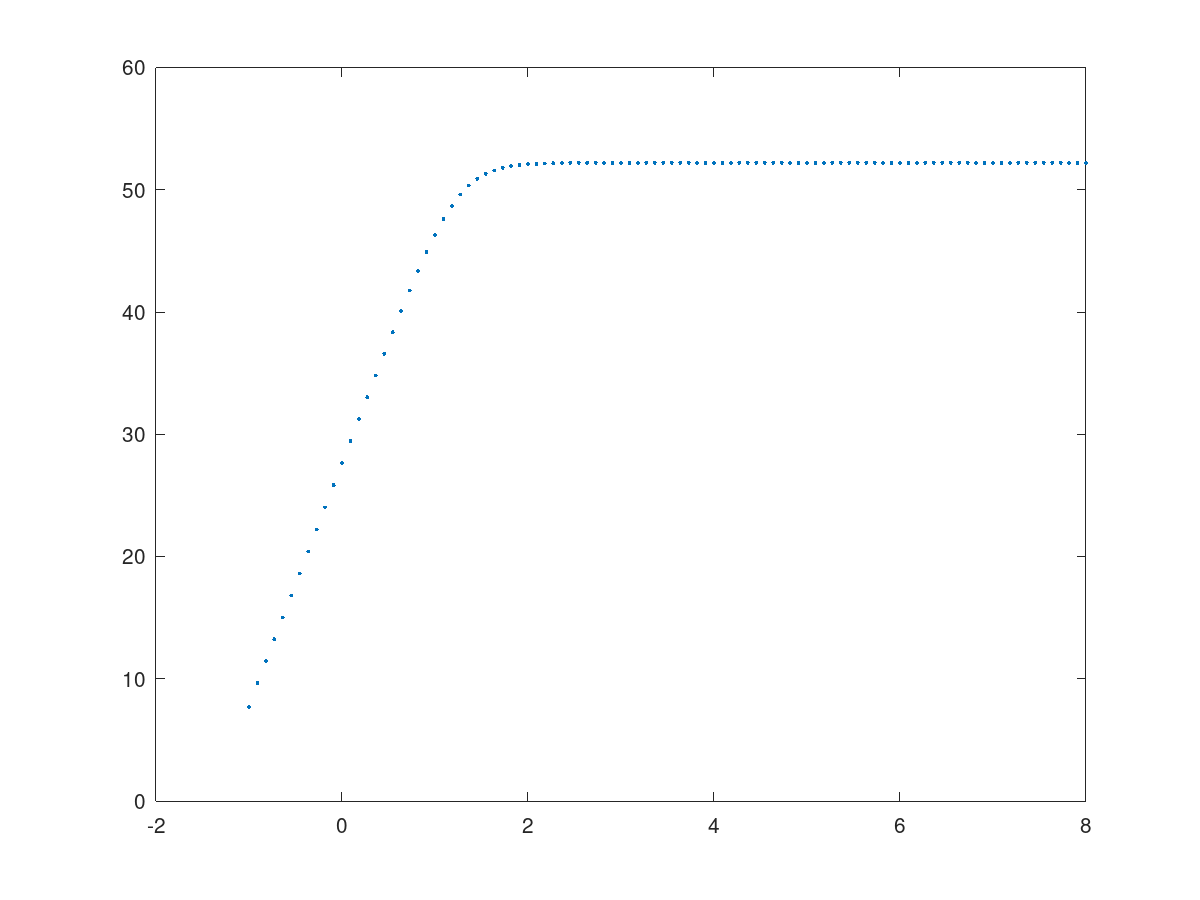
\includegraphics[width=\linewidth]{GAINVERDADEIRO.png}
  \caption{Frequency response of Voltage gain in Gain stage}
  \label{fig:theoplots}
  \endminipage\hfill
\end{figure}




